%
% This is the LaTeX template file for lecture notes for EE 382C/EE 361C.
%
% To familiarize yourself with this template, the body contains
% some examples of its use.  Look them over.  Then you can
% run LaTeX on this file.  After you have LaTeXed this file then
% you can look over the result either by printing it out with
% dvips or using xdvi.
%
% This template is based on the template for Prof. Sinclair's CS 270.

\documentclass[twoside]{article}
\usepackage{graphics}
\usepackage{graphicx}
\usepackage{hyperref}
\setlength{\oddsidemargin}{0.25 in}
\setlength{\evensidemargin}{-0.25 in}
\setlength{\topmargin}{-0.6 in}
\setlength{\textwidth}{6.5 in}
\setlength{\textheight}{8.5 in}
\setlength{\headsep}{0.75 in}
\setlength{\parindent}{0 in}
\setlength{\parskip}{0.1 in}

%
% The following commands set up the lecnum (lecture number)
% counter and make various numbering schemes work relative
% to the lecture number.
%
\newcounter{lecnum}
\renewcommand{\thepage}{\thelecnum-\arabic{page}}
\renewcommand{\thesection}{\thelecnum.\arabic{section}}
\renewcommand{\theequation}{\thelecnum.\arabic{equation}}
\renewcommand{\thefigure}{\thelecnum.\arabic{figure}}
\renewcommand{\thetable}{\thelecnum.\arabic{table}}

%
% The following macro is used to generate the header.
%
\newcommand{\lecture}[4]{
   \pagestyle{myheadings}
   \thispagestyle{plain}
   \newpage
   \setcounter{lecnum}{#1}
   \setcounter{page}{1}
   \noindent
   \begin{center}
   \framebox{
      \vbox{\vspace{2mm}
    \hbox to 6.28in { {\bf EE 382C/361C: Multicore Computing
                        \hfill Fall 2016} }
       \vspace{4mm}
       \hbox to 6.28in { {\Large \hfill Lecture #1: #2  \hfill} }
       \vspace{2mm}
       \hbox to 6.28in { {\it Lecturer: #3 \hfill Scribe: #4} }
      \vspace{2mm}}
   }
   \end{center}
   \markboth{Lecture #1: #2}{Lecture #1: #2}
   %{\bf Disclaimer}: {\it These notes have not been subjected to the
   %usual scrutiny reserved for formal publications.  They may be distributed
   %outside this class only with the permission of the Instructor.}
   \vspace*{4mm}
}

%
% Convention for citations is authors' initials followed by the year.
% For example, to cite a paper by Leighton and Maggs you would type
% \cite{LM89}, and to cite a paper by Strassen you would type \cite{S69}.
% (To avoid bibliography problems, for now we redefine the \cite command.)
% Also commands that create a suitable format for the reference list.
\renewcommand{\cite}[1]{[#1]}
\def\beginrefs{\begin{list}%
        {[\arabic{equation}]}{\usecounter{equation}
         \setlength{\leftmargin}{2.0truecm}\setlength{\labelsep}{0.4truecm}%
         \setlength{\labelwidth}{1.6truecm}}}
\def\endrefs{\end{list}}
\def\bibentry#1{\item[\hbox{[#1]}]}

%Use this command for a figure; it puts a figure in wherever you want it.
%usage: \fig{NUMBER}{SPACE-IN-INCHES}{CAPTION}
\newcommand{\fig}[3]{
			\vspace{#2}
			\begin{center}
			Figure \thelecnum.#1:~#3
			\end{center}
	}
% Use these for theorems, lemmas, proofs, etc.
\newtheorem{theorem}{Theorem}[lecnum]
\newtheorem{lemma}[theorem]{Lemma}
\newtheorem{proposition}[theorem]{Proposition}
\newtheorem{claim}[theorem]{Claim}
\newtheorem{corollary}[theorem]{Corollary}
\newtheorem{definition}[theorem]{Definition}
\newenvironment{proof}{{\bf Proof:}}{\hfill\rule{2mm}{2mm}}

% **** IF YOU WANT TO DEFINE ADDITIONAL MACROS FOR YOURSELF, PUT THEM HERE:

\begin{document}
%FILL IN THE RIGHT INFO.
%\lecture{**LECTURE-NUMBER**}{**DATE**}{**LECTURER**}{**SCRIBE**}
\lecture{5}{September 8}{Vijay Garg}{Nishanth Shanmugham}
%\footnotetext{These notes are partially based on those of Nigel Mansell.}

% **** YOUR NOTES GO HERE:

\section{Topics}

The topics covered in this lecture are:
\begin{itemize}
    \item Semaphores
    \begin{itemize}
        \item Why / what / motivation
        \item Usage
        \item Implementation
        \item Java code on GitHub
        \begin{itemize}
            \item BinarySemaphore
            \item CountingSemaphore
        \end{itemize}
    \end{itemize}
    \item Consumer-producer problem
    \item Reader-writer problem
    \item Dining philosopher's problem
\end{itemize}

\section{Semaphores}

Semaphores provide a means to achieve mutual exclusion.

\subsection{Why / what / motivation}

Think back to Peterson's algorithm. We performed a busy-wait: \\\\
\texttt { while (wantCS[1] \&\& (turn == 1)) \{ no\_op(); \}}

This wait consumes the CPU while waiting for the condition to become false. So core execution time is wasted. This busy-wait can be avoided with help from the operating system.

So how does the OS schedule threads?

\begin{figure}
  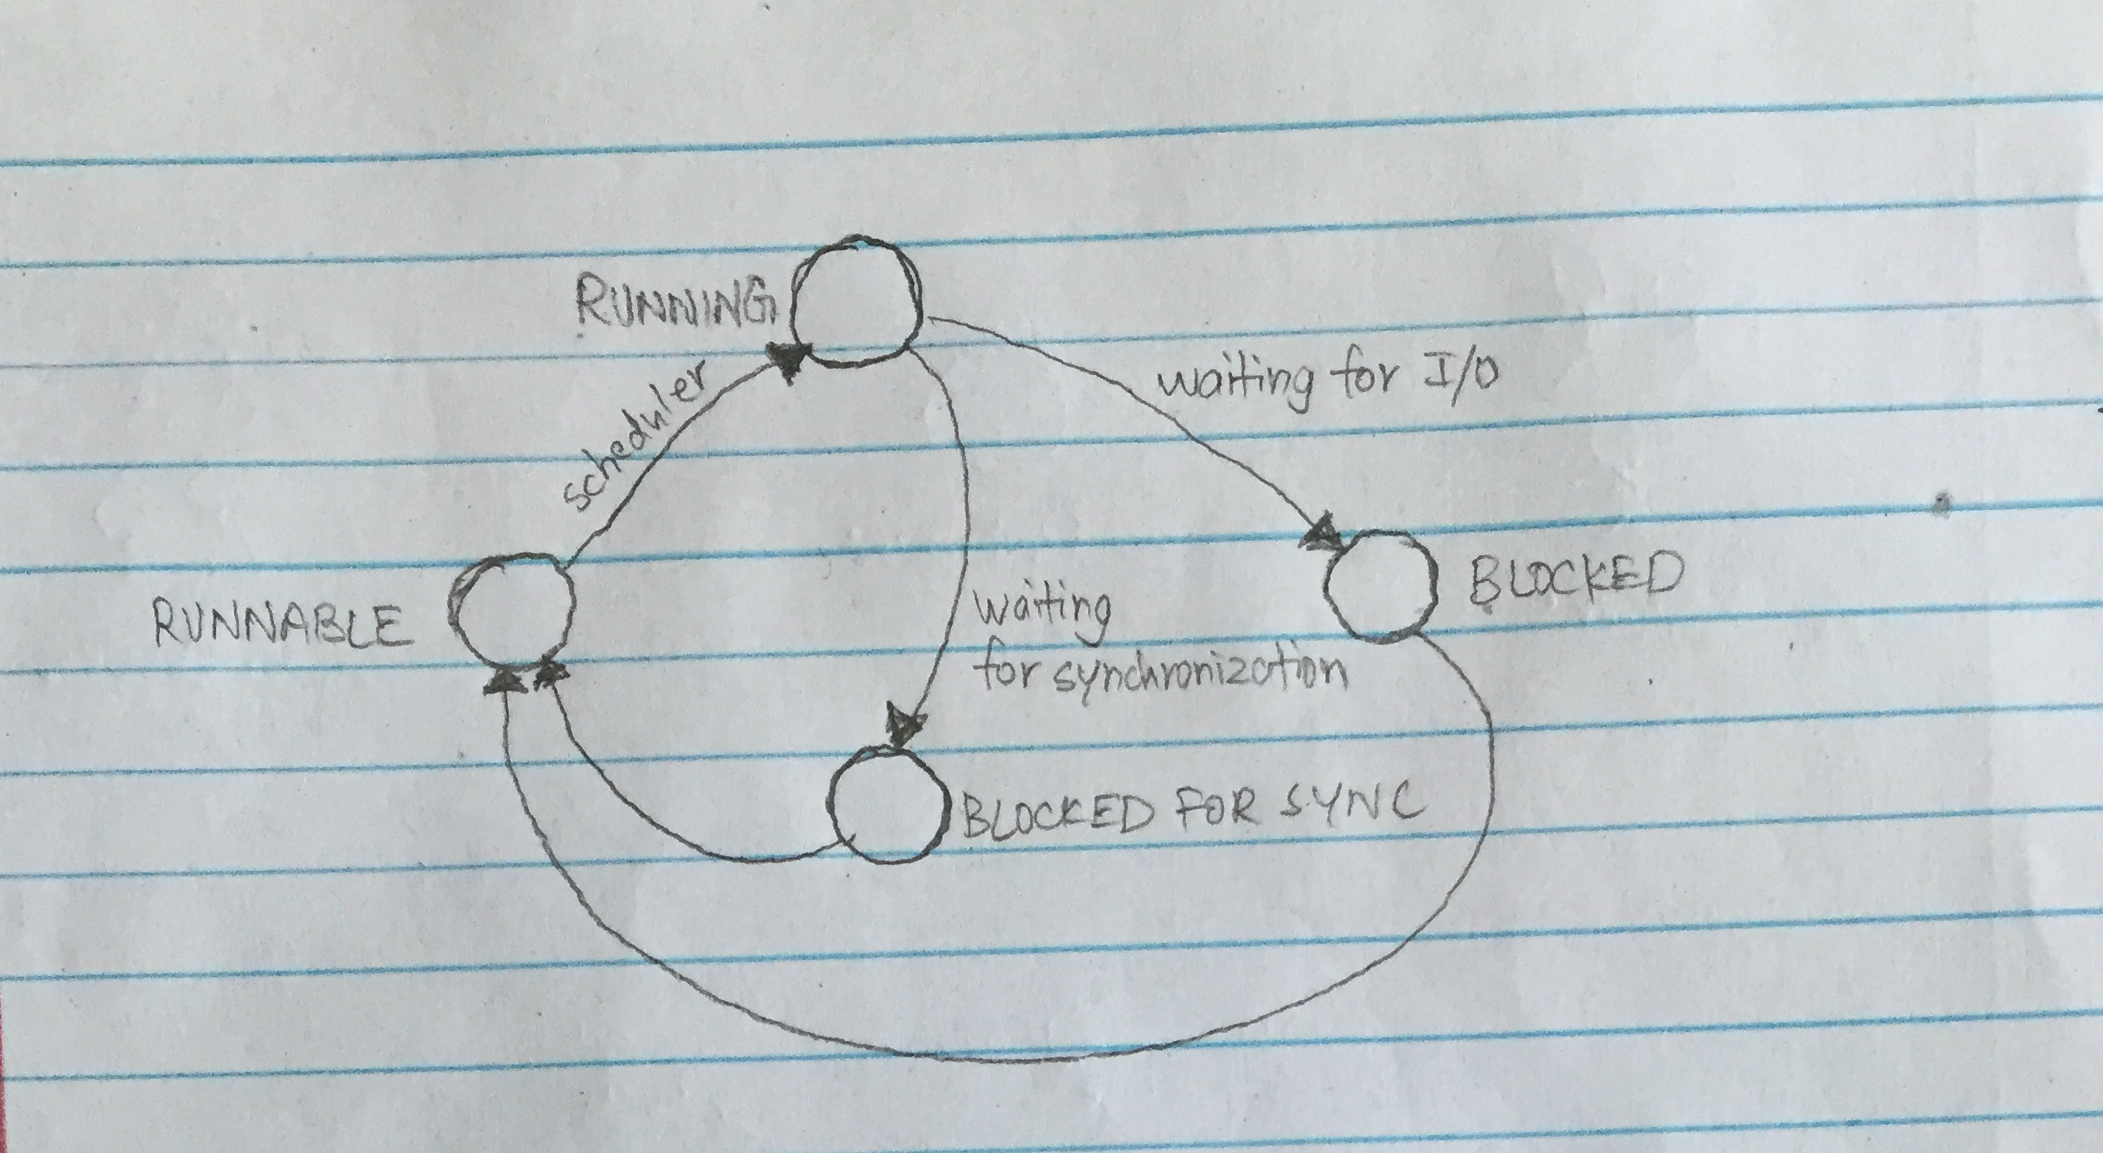
\includegraphics[width=\linewidth]{img/states.png}
  \caption{OS scheduling queues}
\end{figure}

\begin{itemize}
    \item The scheduler puts \textsc{Runnable} threads to \textsc{Running} queue.
    \item If a \textsc{Running} thread issues a blocking call (for example, I/O) then it is put in \textsc{Blocked} queue.
    \item Once the I/O operation returns, the blocked thread can be scheduled for running again by putting in the \textsc{Runnable} queue.
    \item Similarly, instead of running no\_op()'s, the OS should be able to take it out of the \textsc{Running} queue and put into the \textsc{Blocked} queue waiting for synchronization.
\end{itemize}

\subsection{Usage}

Semaphores were introduced by Dijkstra in {\it The Operating System}. A semaphore has two operations defined on it:

\begin{itemize}
    \item P(), or acquire()
    \item V(), or release()
\end{itemize}

That is, if {\tt s} is a semaphore then {\tt s.P()} and {\tt s.V()} are the two possible calls.

\subsection{Visualization}

A simple way to visualize to semaphore is as a bottle with a marble inside it. The marble could either be present inside the bottle or not inside it the bottle.

\begin{figure}
  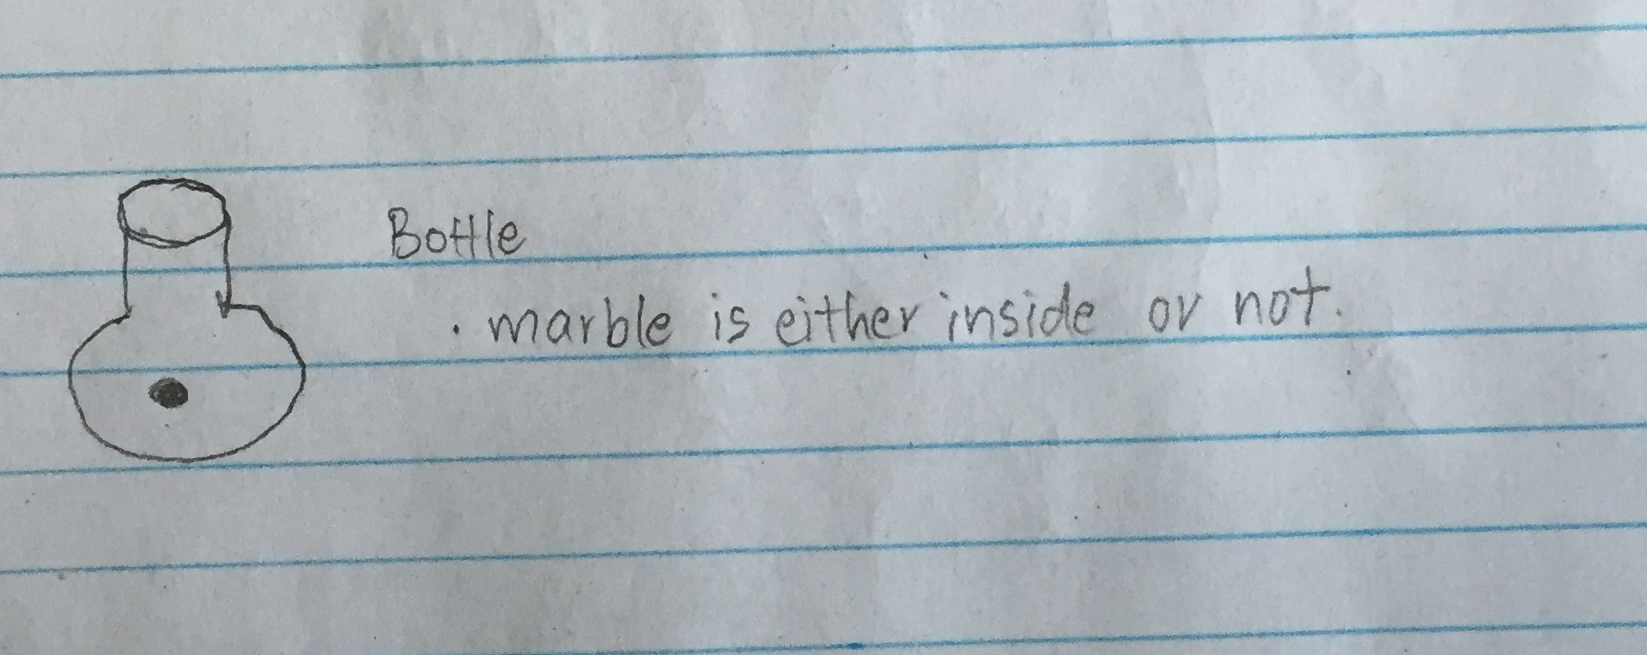
\includegraphics[width=\linewidth]{img/bottle.png}
  \caption{Semaphore}
\end{figure}

If a thread wishes to enter a critical section, it should first obtain the marble before it proceeds to enter the CS.
If the marble is present, it removes the marble and proceeds to enter the CS.
If the marble is not present, it waits until the marble is present to try again.

The {\tt value} variable in the implementation below corresponds to the marble.

\subsection{Implementation}

A semaphore has one field:

{\tt value: boolean, initially true }

The implementation for {\tt P()} is below. Note that both lines would need to execute atomically.

{\tt while (!value) \{ wait(); \}\\
value = false;}

The implementation for {\tt V()} is:

{\tt value = true; }

\subsection{Discussion}

But isn't it weird that we have to perform P() atomically? Essentially, it appears like we need to use mutual exclusion to build mutual exclusion.

We will have to use busy-wait to achieve atomicity of P().

\begin{itemize}
    \item For programmer's CS, we will use semaphore.
    \item For semaphore's CS, we will use busy-wait.
\end{itemize}

This is an okay compromise. The reason to not use busy-wait for programmer's CS are that programmer's CS are generally longer and may contain bugs in the implementation. On the other hand, semaphore's CS is known to be small. Thus using a semaphore saves system resources.

\subsubsection{notify}

Sometimes, it might be necessary to wake up one of the sleeping threads once the current threads completes it work in the CS. For this, we use {\tt notify()}. The {\tt notify() } call does not guarantee the order in which threads are woken up---it simply wakes up any one thread. 
\\\\
To guarantee order, Java provides a fairness parameter. But generally, it is good practice to not expect order guarantees in concurrent programs that do not require ordering.

\subsubsection{Monitors}

Semaphores might hinder code readability since semaphores are used for both {\it mutual exclusion} and {\it conditional execution}. In addition:

\begin{itemize}
    \item The order of {\tt P()} calls is important to avoid deadlocks.
    \item {\tt P()} calls should be paired with corresponding {\tt V()} calls to avoid deadlocks.
\end{itemize}

Monitors provide a suitable mechanism to handle these, but are explored in a future lecture.

\subsection{Java code}
\subsubsection{BinarySemaphore}

The \href{https://github.com/vijaygarg1/UT-Garg-EE382C-EE361C-Multicore/blob/master/chapter3-synchronization_primitives/BinarySemaphore.java}{{\tt BinarySemaphore}} class on GitHub implements the kind of semaphore described above.

Of note, the Util.myWait call on line 8 puts the current thread in the blocked queue. Also, the synchronized keyword in the method signatures guarantee that only one thread is executing the method at any given time. This provides the required atomicity.

\subsubsection{CoutingSemaphore}

\href{https://github.com/vijaygarg1/UT-Garg-EE382C-EE361C-Multicore/blob/master/chapter3-synchronization_primitives/CountingSemaphore.java}{{\tt CountingSemaphore}} allows multiple threads to be in the CS at a given time. The value field is now an int instead of a boolean.

\section{Producer-consumer problem}

\subsection{Description}

There is a producer thread and a consumer thread. The producer deposits to shared buffer, and the consumer reads from the shared buffer. The constraints are:

\begin{itemize}
    \item Mutual exclusion (no concurrent read/write to shared buffer)
    \item Conditional synchronization. The consumer has to wait for buffer to be non-empty before read; the producer has to wait for buffer to be non-full before depositing.
\end{itemize}

\begin{figure}
  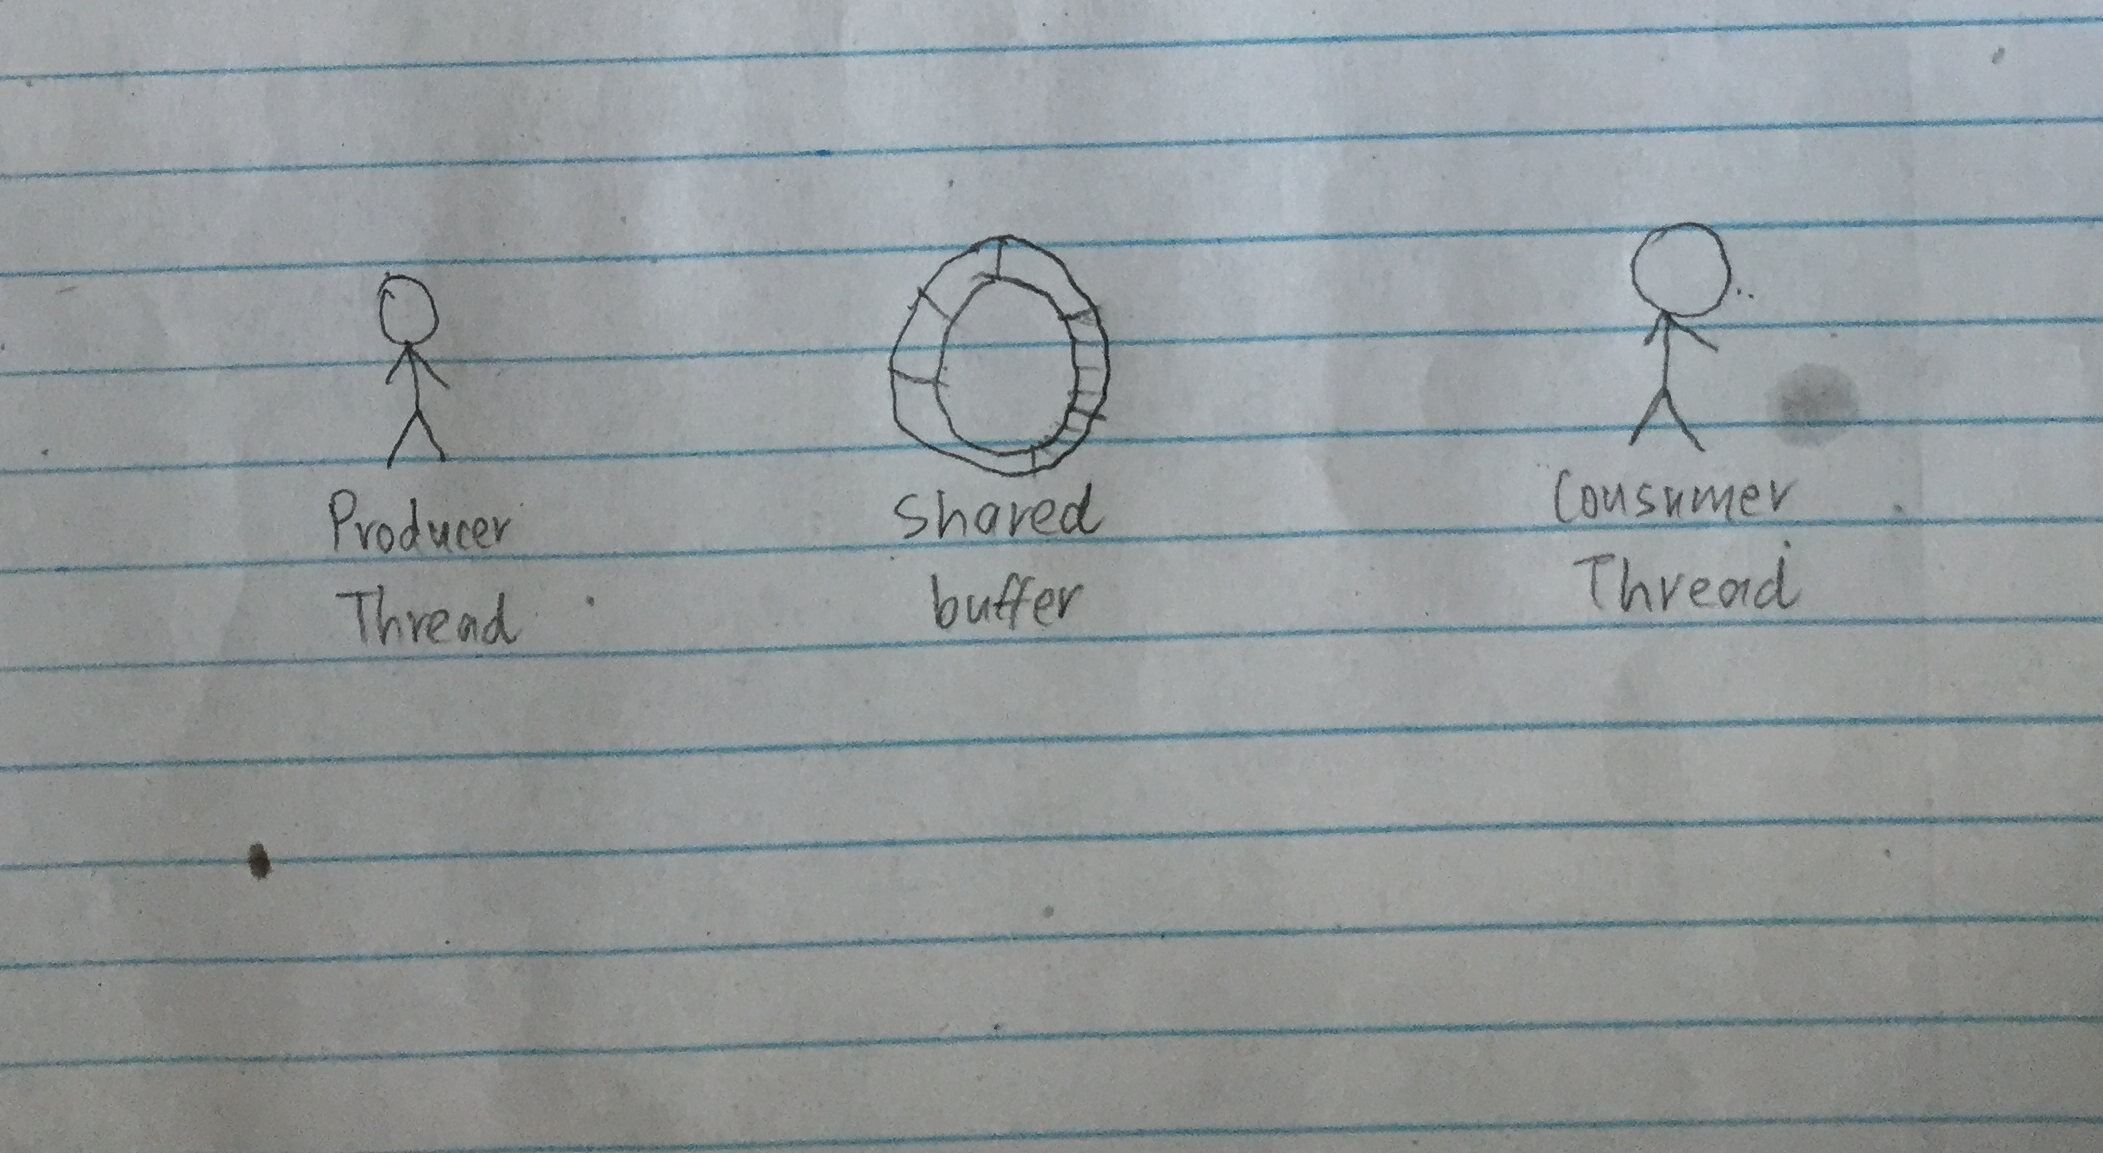
\includegraphics[width=\linewidth]{img/prodcon.png}
  \caption{Producer-consumer}
\end{figure}

\subsection{Implementation}

\href{https://github.com/vijaygarg1/UT-Garg-EE382C-EE361C-Multicore/blob/master/chapter3-synchronization_primitives/BoundedBuffer.java}{{\tt BoundedBuffer}} class on GitHub contains a solution to this problem. The noteworthy observations from the code are:

\begin{itemize}
    \item The mutex is a BinarySemaphore. It is a common convetion to use a BinarySemaphore for mutual exclusion.
    \item The conditional synchronization is provided by the CountingSemaphores, namely {\tt isEmpty} and {\tt isFull}.
    \item The other thread is woken up / notified by the {\tt V()} calls on lines 15 and and 24.
\end{itemize}

Question: Is it okay to change the order of the calls on lines 10 and 11? No, here's an example execution order that results in deadlock if the order was changed.

\begin{itemize}
    \item The buffer is full. The producer grabs the mutex. Then the producer waits for the buffer to be not full so that it can deposit.
    \item The condition that the producer is waiting for will never be fulfilled.
    \item This is because the consumer will not be able to consume from the buffer, because the mutex is held by the producer.
\end{itemize}

In the correct order of code on GitHub, this will not happen because consumer and producer only grab the mutex if their entry conditions are already satisfied.

\section{Reader-writer problem}

\subsection{Description}

The problem aims to establish a protocol for multiple readers and writers to safely access a shared database. The constraints are:

\begin{itemize}
    \item No read-write conflict.
    \item No write-write conflict.
    \item Read-read conflict is allowed.
    \item There is no need to guarantee starvation freedom for writers. It is okay for readers to read repeatedly.
\end{itemize}

\subsection{Implementation}

\href{https://github.com/vijaygarg1/UT-Garg-EE382C-EE361C-Multicore/blob/master/chapter3-synchronization_primitives/ReaderWriter.java}{{\tt ReaderWriter}} class on GitHub contains a solution to this problem.

The {\tt startWrite} and {\tt startRead} methods are the entry protocol for writers and readers respectively. Similary, {\tt endWrite} and {\tt endRead} are the exit protocols for writers and readers respectively.

{\tt startWrite} and {\tt endWrite} are simple. Writers simply need to acquire {\tt wlock} before they can write and release it when done writing. The acquiring of the BinarySemaphore wlock ensures that only one writer is writing at any given time.

Readers on the other hand need to ensure that no writers exist before they can read. The first reader to enter has to wait until all writers leave. When the first reader enters it grabs the wlock (line 8) ensuring no writers can enter until the last exiting readers release wlock (line 14). Readers after the first reader simply need to enter and exit. The last reader to exit has to release wlock as described before.

To track the number of readers, the numReaders variable is used. It is incremented on entry and decemented on exit. It is guarded by mutex to prevent concurrent modification of the variable by readers.

\begin{figure}
  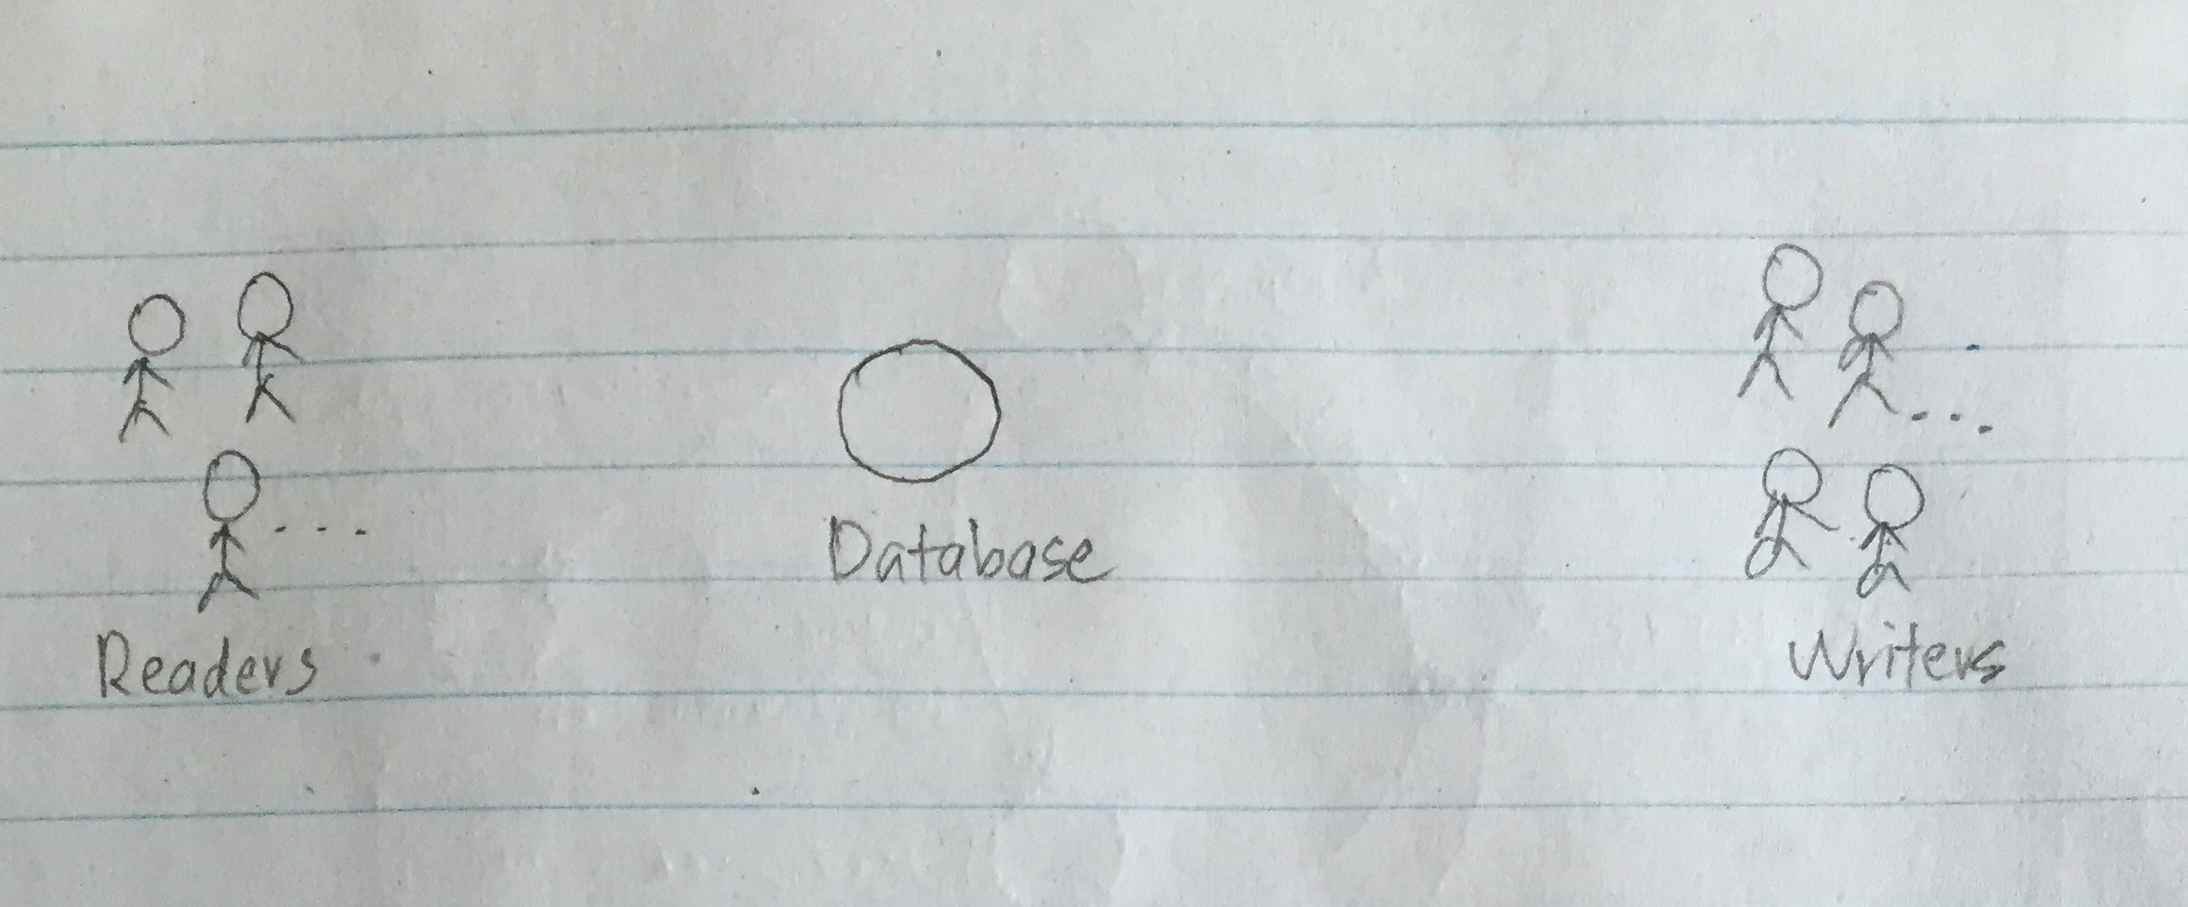
\includegraphics[width=\linewidth]{img/rw.png}
  \caption{Reader-writer}
\end{figure}

\section{Dining philosophers problem}

\subsection{Description}

n philosophers sit around a circular dining table.  There are n forks placed in between the philosophers. To eat, a philosopher requires two forks---the one of her left and the one of her right.

\begin{figure}
  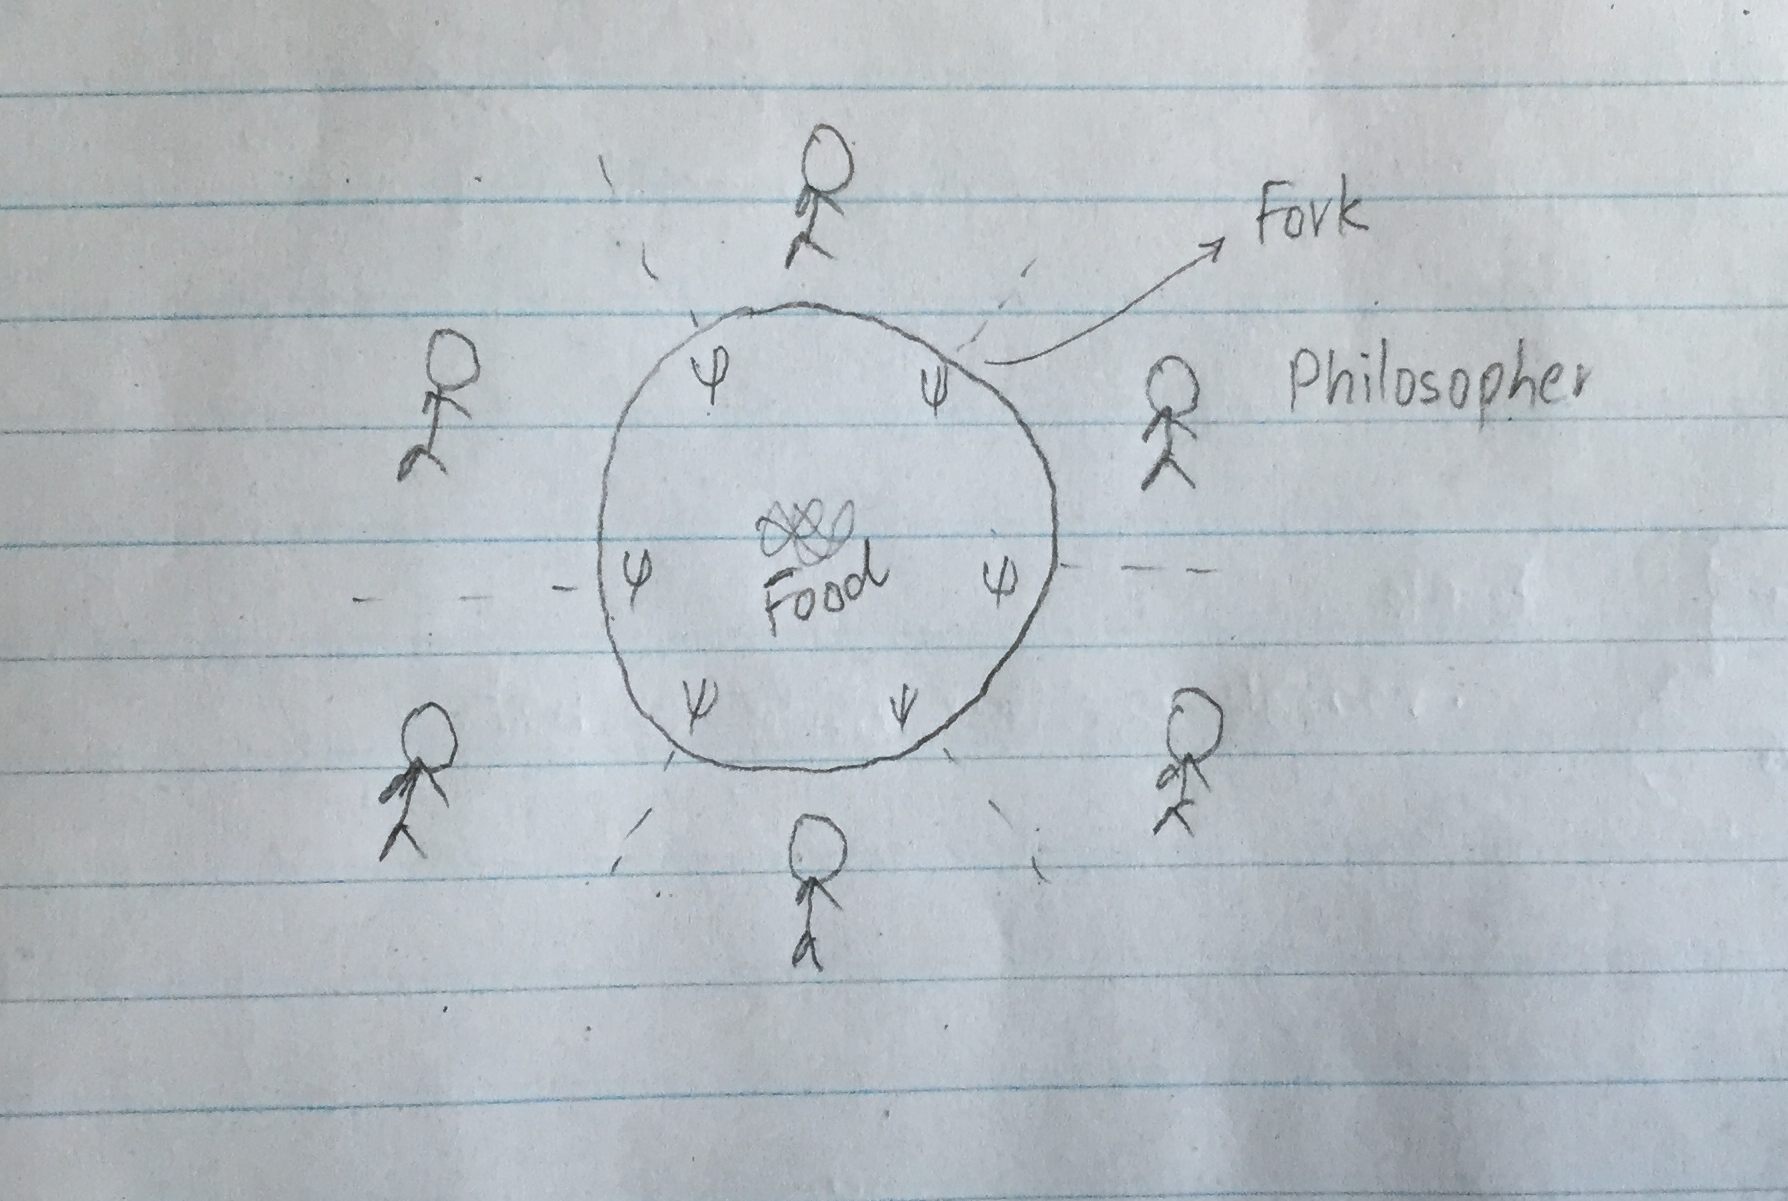
\includegraphics[width=\linewidth]{img/phil.png}
  \caption{Dining philosophers}
\end{figure}

Philosophers switch between these states in order: {\it thinking} to {\hungry}, {\it hungry} to {\it eating}, and {\it eating} back to {\it thinking}.

The goal is to design a protocol with the following constraint: Two neighboring philosophers cannot eat at the same time.

Philosophers should use an {\tt acquire} call to acquire forks and a {\tt release} call when done eating.

The \href{https://github.com/vijaygarg1/UT-Garg-EE382C-EE361C-Multicore/blob/master/chapter3-synchronization_primitives/Philosopher.java}{Philosopher} class on GitHub represents a philosopher. \href{https://github.com/vijaygarg1/UT-Garg-EE382C-EE361C-Multicore/blob/master/chapter3-synchronization_primitives/DiningPhilosopher.java}{DiningPhilosopher} provides a simple (but incorrect) implementation of Resource.

It is incorrect because it can result in a deadlock. In the acquire method, philosopher's first grab the left fork then the right fork. In a circular dining table, it could happen that the philosophers all grab their left fork first. When the philosophers now try to obtain the right fork, they will fail to do so because it has been obtained by their neighbor to the right (who grabbed it initially as her left fork). 

This is problem arises because of symmetry.

\subsubsection{Fixes}

Possible fixes to the DiningPhilosopher class are listed below.

\begin{itemize}
    \item Breaking symmetry: exactly one philosopher will be instructed to grab her right fork before the left. This will prevent the deadlock.
    \item Restrict number of philosophers that can be eating at any given time to less than n: For instance, there could be a precursor step of standing up before acquiring a fork. At that point, we can restrict that at most less than n philosophers can be standing at any instant.
\end{itemize}

\section*{References}
\beginrefs
\bibentry{GitHub}{} Multicore source code, {\it https://github.com/vijaygarg1/UT-Garg-EE382C-EE361C-Multicore}
\endrefs


\end{document}
